\documentclass[12pt,a4paper]{ctexart} 

% ---------- 宏包加载 ----------
\usepackage{amsmath,amssymb}          % 数学符号与公式
\usepackage{graphicx}                 % 插图
\graphicspath{{./}{figures/}}
\usepackage{booktabs}                 % 三线表
\usepackage{tabularx}                 % 自适应表格
\usepackage{makecell}                 % 表格内换行
\usepackage{algorithm}                % 算法浮动体
\usepackage{algorithmic}              % 算法伪代码
\usepackage{url}                       % 网址引用
\usepackage{xcolor}                    % 颜色支持
\usepackage{geometry}                  % 页面设置
\usepackage{mathrsfs}                  % 花体符号
\usepackage{amsthm}
\theoremstyle{definition}
\newtheorem{definition}{定义}[section]
\newtheorem{assumption}{假设}[section]
\theoremstyle{plain}
\newtheorem{theorem}{定理}[section]
\newtheorem{lemma}{引理}[section]
\newtheorem{proposition}{命题}[section]
\newtheorem{corollary}{推论}[section]
\geometry{left=2.5cm,right=2.5cm,top=2.5cm,bottom=2.5cm}
\renewenvironment{abstract}{
  \centerline{\textbf{摘\quad要}}\vspace{0.5em}\noindent
}{\par\vspace{1em}}
\usepackage{hyperref}                  % 超链接
\hypersetup{
    colorlinks=true,
    linkcolor=black,
    citecolor=black,
    urlcolor=blue
}

\pagestyle{plain}                     % 移除页眉，只保留页码

% ---------- 自定义命令 ----------
\newcommand{\keywords}[1]{\noindent\textbf{关键词：} #1} % 关键词命令

% ---------- 标题信息 ----------
\title{\textbf{推荐系统中的数据资产价值评估——基于训练动力学的梯度流代理指标}}


\begin{document}

\date{}
\maketitle

% ---------- 摘要 ----------
\begin{abstract}
随着数据要素市场的加速建设，推荐系统中的数据资产价值计量已成为数字经济治理的核心难题。深度推荐模型将多源异构行为数据压缩为排序或匹配预测输出，导致系统性能改进与微观数据单元贡献之间的因果链条难以直接追溯，进而引发数据资产"有值难量、可用难价"的管理困境。本文提出一个基于训练动力学的数据价值评估框架，在不依赖重复重训练的前提下实现对数据单元贡献的可计算度量。

方法上，本文将瞬时数据影响定义为验证损失梯度与样本梯度的内积，并沿随机梯度下降训练轨迹进行学习率加权累积，得到数据价值流（Data Value Flow, DVF），以刻画数据对泛化能力的时变作用；进一步给出训练阶段分解，区分表示学习与目标对齐阶段的差异化贡献。在理论层面，本文证明了DVF在满足连续性、路径可加性与局部一致性三条公理的数据价值函数类中具有唯一性，并阐明其与影响函数、TracIn及数据Shapley值之间的统一关系。在标准收敛假设下，本文推导出闭式代理指标——SGD影响流（SGD Influence Flow, SIF）及其曲率修正版本SIF+，将估值复杂度由轨迹累积形式降至一次验证梯度与样本梯度内积的可部署形式，总计算复杂度仅为$O(Nd)$，相比TracIn与DVF所需的完整轨迹累积（耗时约27.9秒）降低约25倍，SIF仅需约1.1秒即可完成全量样本估值。

实验上，本文采用统一数据处理与评测协议，以MLP基准模型在MovieLens1M、Yahoo!Music与Pinterest三类公开数据集上完成可复现实证，比较SIF、SIF+、Influence Function、DVF与TracIn在deletion/insertion/NDCG曲线、随机基线校正指标、运行开销及5个随机种子统计检验下的表现。实验结果表明：SIF取得Deletion-AUC $0.0669\pm0.0248$、Insertion-AUC $0.1419\pm0.0334$、NDCG@Ke-AUC $33.75\pm4.42$；SIF+在归因质量上进一步提升，Deletion-AUC达$0.0683\pm0.0209$、Insertion-AUC达$0.1513\pm0.0216$、NDCG@Ke-AUC达$35.43\pm2.80$，标准差更小，稳定性更优；而Influence Function的Deletion-AUC仅为$-0.0091\pm0.0066$，归因效果明显偏弱。Wilcoxon检验与Holm校正结果显示，SIF/SIF+与DVF、TracIn之间差异不显著（$p=1.000$），但SIF/SIF+的运行耗时仅为后两者的约$\frac{1}{25}$，在归因质量与计算成本之间呈现显著更优的折中。本文最后讨论了框架在合规前提下用于数据资产仪表盘的应用潜力，并给出持续更新的后续验证路径。
\end{abstract}


\keywords{推荐系统；数据资产；数据价值评估；训练动力学；数据价值流（DVF）；SGD影响流（SIF）；TracIn；影响函数；数据Shapley；因果归因基线}

% ---------- 目录 ----------
\newpage
\tableofcontents
\newpage

% ---------- 引言 ----------
\section{引言}
\label{sec:intro}
随着《中华人民共和国个人信息保护法》《中华人民共和国数据安全法》等法律法规的相继出台，以及《中共中央 国务院关于构建数据基础制度更好发挥数据要素作用的意见》明确提出将数据要素作为推动数字经济发展的关键资源，数据资产的管理与价值计量已成为企业数字化转型的核心议题。然而，在推荐系统中，以深度兴趣网络\cite{zhou2018deep}为代表的深度模型将高维行为数据压缩为排序或匹配预测，使系统效益改进与底层数据单元之间的因果关系呈现明显“黑箱”特征。传统资产估值方法（成本法、收益法、市场法）因数据资产的非实体性、价值易变性与强情境依赖而难以直接适配\footnote{参见《加快构建数据资产估值体系 赋能数字经济发展》，\url{https://www.deo.org.cn/article/hygd_sjpg/detail143.html}}。如何在合规框架下对数据要素进行可计算的价值度量，已成为数据市场与数据治理领域的重要研究议题\cite{xu2023data}。

在上述背景下，本文将问题先收敛到\textbf{归因层}，即先回答“哪些数据单元在模型泛化中产生了可重复、可解释的边际影响”。这样处理主要基于三点考虑。首先在方法层面，样本梯度与验证梯度可形成可计算的局部影响代理，便于在统一训练轨迹下进行重复检验。在工程层面，归因指标可以直接复用既有检查点与验证流程，减少为单一估值任务进行大规模重训练的成本。在治理层面，归因结论更容易附带统计边界与不确定性说明，也更符合“先证据、后决策”的审慎披露要求。基于这一思路，本文将“归因可信度”作为连接模型效果与数据价值讨论的起点。

学术界已提出多类数据价值评估方法，但各有其局限。基于合作博弈的数据Shapley值\cite{ghorbani2019data}具有严格的公平性公理保证，但其精确计算需枚举所有$2^N$个数据子集，已被证明为$\#P$-hard问题\cite{andos2012computation}，在现代深度推荐模型中完全不可行。影响函数\cite{influence}通过局部二阶近似将"删除样本"操作转化为连续可微的权重扰动问题，无需重训练即可估计样本影响，但其依赖精确Hessian逆矩阵的计算——对于参数量达$10^7$量级的推荐模型，存储完整Hessian需$O(d^2)$空间，求逆需$O(d^3)$时间，工程上难以落地。TracIn\cite{TracIn}通过沿训练轨迹累积梯度内积估计样本影响，避免了Hessian求逆，但需保存完整训练轨迹或多个检查点，计算开销仍然较高（本文实验中耗时约27.9秒/次），且未能区分不同训练阶段的差异化贡献。上述方法的共同局限在于：它们或将训练过程视为静态黑箱，或在计算效率与估值精度之间存在难以调和的矛盾，难以满足工业级推荐系统对"实时、可解释、可部署"数据价值监控的需求。

在上述背景下，本文将问题先收敛到\textbf{归因层}，即先回答"哪些数据单元在模型泛化中产生了可重复、可解释的边际影响"。这样处理主要基于三点考虑：在方法层面，样本梯度与验证梯度可形成可计算的局部影响代理，便于在统一训练轨迹下进行重复检验；在工程层面，归因指标可直接复用既有检查点与验证流程，减少为单一估值任务进行大规模重训练的成本；在治理层面，归因结论更容易附带统计边界与不确定性说明，符合"先证据、后决策"的审慎披露要求。

本文的核心贡献体现在以下四个方面：

\textbf{（1）公理化理论框架。}本文提出路径依赖数据价值（PDV）的公理体系，证明在连续性、路径可加性与局部一致性三条自然公理下，基于训练轨迹梯度内积的价值函数在常数缩放意义下唯一，从而将数据价值评估从经验性构造提升为具有理论保证的公理化定义。

\textbf{（2）统一理论视角。}本文在同一框架下阐明DVF与影响函数、TracIn及数据Shapley值之间的关系：TracIn是DVF的离散特例，影响函数是PDV的局部二阶近似，数据Shapley值在梯度流极限与线性化假设下与DVF期望形式等价。这一统一视角揭示了现有方法的内在联系，并为方法选择提供了理论依据。

\textbf{（3）高效可部署的SIF/SIF+指标。}在标准收敛假设下，本文推导出闭式代理指标SIF（SGD Influence Flow）及其曲率修正版本SIF+。SIF将估值复杂度降至$O(Nd)$，仅需一次验证梯度计算与逐样本内积，运行耗时约1.1秒，相比DVF/TracIn的约27.9秒提速约25倍，同时在归因质量上与后两者无显著差异（Wilcoxon检验，Holm校正后$p=1.000$）。SIF+通过对角Hessian近似引入曲率修正，在保持$O(Nd)$总复杂度的同时进一步提升估值稳定性（NDCG@Ke-AUC标准差由4.42降至2.80），在归因质量与计算成本之间实现了更优折中。

\textbf{（4）可复现的实证评测体系。}本文建立统一数据处理与评测协议，在MovieLens1M、Yahoo!Music与Pinterest三类公开数据集上，以deletion/insertion/NDCG曲线、随机基线校正指标与多随机种子统计检验（Wilcoxon + Holm校正 + Cliff's $\delta$效应量）联合评估各方法，提供趋势性实证证据，并开源全部代码与数据处理流程\cite{repository}以支持复现。


本研究关注“深度归因—价值反演”，穿透模型黑箱，将系统层面的性能增量公平、可解释地归因至微观数据单元，从而支持数据治理与价值配置。具体而言，本文试图回答以下问题：在基于深度学习的推荐系统中，如何量化并验证不同价值密度的数据单元对模型泛化效用的公平贡献比例？

\begin{figure}[H]
    \centering
    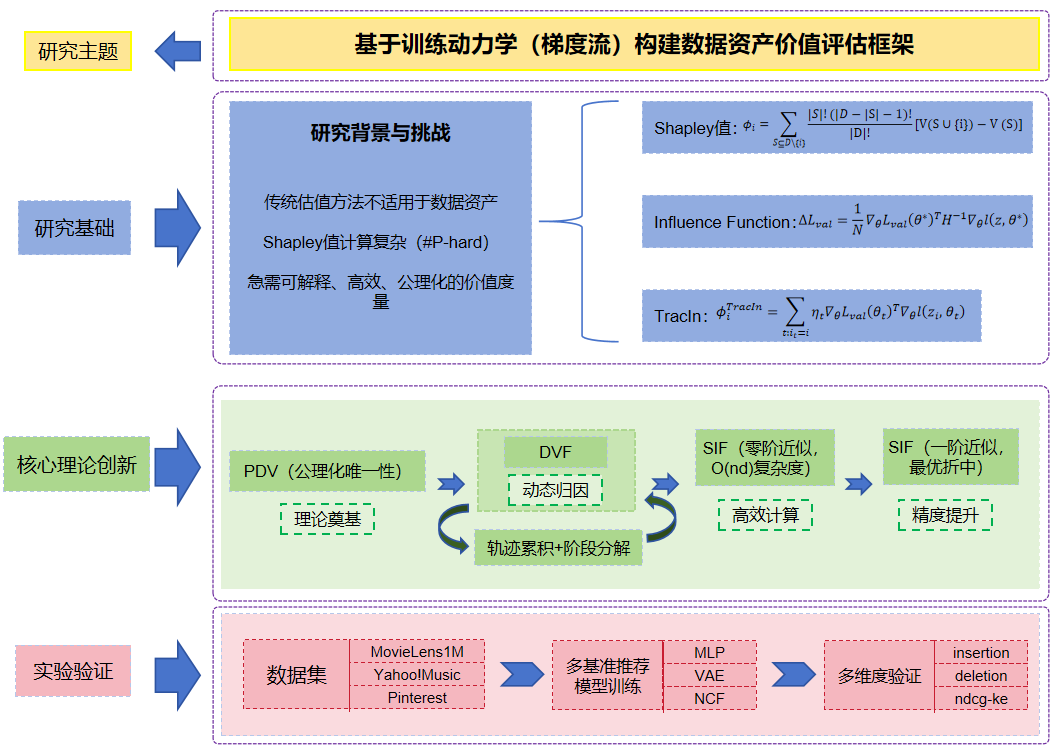
\includegraphics[width=0.8\textwidth]{figures/Summary.png}
    \caption{本研究的框架概述}
    \label{fig:summary}
\end{figure}

% ---------- 相关工作与问题分析 ----------
\section{相关工作与问题分析}
\label{sec:related}
数据价值评估（Data Valuation）旨在量化单个数据样本或数据子集对机器学习模型性能的贡献，是近年来机器学习系统、数据市场和数据治理领域的重要研究方向。现有方法大体可分为三类：基于合作博弈的Shapley值方法、基于验证集损失和训练集损失的影响函数（Influence Function）的方法，以及基于梯度下降的TracIn方法。

\subsection{问题形式化}
\label{sec:problem_formalization}
考虑一个深度推荐模型 $f$，输入特征集合 $D = \{U, I, C\}$，其中 $U$ 为用户侧特征，$I$ 为商品侧特征，$C$ 为上下文特征。模型输出预测值 $\hat{y} = f(D)$，具体形式可以是点击概率（CTR）、转化概率（CVR）或期望GMV等。平台在统计周期内观测到的总收益为 $\text{GMV}_{\text{model}} = \sum \hat{y}$。

定义随机推荐参考策略下的预期收益为 $\text{GMV}_{\text{random}}$，则AI增量收益为：
\[
\Delta\text{GMV}_{\text{total}} = \text{GMV}_{\text{model}} - \text{GMV}_{\text{random}}.
\]

本文的目标是设计一个价值分配函数 $\text{Valuate}(\cdot)$，将 $\Delta\text{GMV}_{\text{total}}$ 公平地分配给各数据资产单元 $\{d_i\}$，使得分配结果满足公平性公理。

然而，传统方法通常将模型视为静态黑箱，忽略训练动态对数据价值的深刻影响。为此，我们首先回顾基于博弈论的静态归因方法，随后提出一种全新的、能够捕捉训练动力学因果贡献的动态价值反演框架。

\subsection{Shapley-based Data Valuation}
Shapley值最早由Lloyd Shapley于1953年提出\cite{shapley1953value}，用于解决合作博弈中的收益分配问题。Amirata Ghorbani~\cite{ghorbani2019data}首次将其引入机器学习中的数据估值问题，提出Data Shapley框架，通过计算数据点在所有可能数据子集中的边际贡献来定义数据价值。该方法满足效率性、对称性、虚拟性和可加性等公平分配公理，是一种公认的具有理论保证的数据价值定义。

数据点$z_i$的Shapley值定义形式为：
\begin{equation}
\phi_i =\sum_{S \subseteq D\setminus\{i\}}\frac{|S|!(|D|-|S|-1)!}{|D|!}\left[V(S\cup\{i\})-V(S)\right],
\end{equation}

其中$V(S)$表示在子集$S$上训练的模型的效用，通常通过在验证集上的准确率等指标来衡量。

Shapley值的理论性质尽管很吸引人，但精确计算需要评估训练数据的所有$2^n$个子集，这种指数爆炸的时间复杂度对于现代机器学习系统来说在计算上是不可行的。为了缓解这个问题，研究者提出了几种近似算法，例如TMC-Shapley和Group Testing Shapley等方法\cite{jia2019towards}。这些方法通过随机排列或采样策略来估计Shapley值。然而，它们仍然需要在不同的数据子集上反复重新训练模型，导致在大型深度学习任务中产生巨大的计算开销。

Shapley家族的另一个局限性在于，它们将学习算法视为一个静态黑箱，且只关注最终的模型性能。因此，现代优化算法的训练动态过程中蕴含的丰富信息在很大程度上被忽略了。

\subsection{Influence Function-based Methods}
影响函数（Influence Function）最早源于稳健统计，用于分析训练样本的微小扰动对模型参数或预测结果的影响。Pang Wei Koh和Percy Liang~\cite{influence}首次将这一思想引入机器学习，通过近似计算删除单个训练样本对模型预测的影响，从而估计样本的重要性。

具体推导可以从权重扰动的角度出发，考虑在原始训练损失\(L_{\mathrm{train}}(\theta)\)的基础上，将某个训练样本$z_i$的权重增加一个微小量$\epsilon$，新的目标函数变为：
\begin{equation}
\tilde{L}_{\mathrm{train}}(\theta) = L_{\mathrm{train}}(\theta) + \varepsilon \ell(z,\theta)
\end{equation}

令\(\theta^{*}\)为原始损失函数（$\epsilon=0$）的最优解，\(\theta_{\varepsilon}\)为扰动后的最优解。根据优化理论，它满足一阶最优条件:
\begin{equation}
\nabla_{\theta} \tilde{L}_{\mathrm{train}}(\theta_{\varepsilon}) = \nabla_{\theta} L_{\mathrm{train}}(\theta_{\varepsilon}) + \varepsilon \nabla_{\theta} \ell(z_i, \theta_{\varepsilon}) = 0
\end{equation}

由于\(\varepsilon\)是一个微小量，我们可以在\(\varepsilon=0\)处对\(\theta_{\varepsilon}\)进行一阶泰勒展开，即$\theta_{\varepsilon} \approx \theta^{*} + \left.\frac{d\theta}{d\varepsilon}\right|_{\varepsilon=0}\varepsilon$。将\(\theta_{\varepsilon}\)代入上式，得到:
\begin{equation}
\nabla_{\theta} L_{\mathrm{train}}(\theta^{*}) + \varepsilon\nabla_{\theta}^2 L_{\mathrm{train}}(\theta^{*})\left.\frac{d\theta}{d\varepsilon}\right|_{\varepsilon=0} + \varepsilon \nabla_{\theta} \ell(z_i, \theta^{*}) + \varepsilon^2\nabla_{\theta}^2 \ell(z_i, \theta^{*})\left.\frac{d\theta}{d\varepsilon}\right|_{\varepsilon=0}= 0
\end{equation}

其中$\nabla_{\theta}^2 L_{\mathrm{train}}(\theta^{*})$为训练损失的Hessian矩阵$H$。因为$\theta^{*}$是未扰动前的最优解，故\(\nabla_{\theta} L_{\mathrm{train}}(\theta^{*})=0\)。$\varepsilon^2\nabla_{\theta}^2 \ell(z_i, \theta^{*})\left.\frac{d\theta}{d\varepsilon}\right|_{\varepsilon=0}$是二阶小量，可以忽略。最终得到：
\begin{equation}
\left.\frac{d\theta}{d\varepsilon}\right|_{\varepsilon=0} = -H^{-1} \nabla_{\theta} \ell(z_i, \theta^{*})
\end{equation}

这一结果刻画了当样本$z_i$的权重发生微小变化时，模型参数$\theta$的变化趋势。进一步地，若要考察该扰动对验证损失$L_{\mathrm{val}}(\theta)$的影响，可以通过链式法则得到：
\begin{equation}
\left.\frac{d}{d\varepsilon} L_{\mathrm{val}}(\theta_{\varepsilon})\right|_{0} = \nabla_{\theta} L_{\mathrm{val}}(\theta^{*})^{\mathsf{T}} \left.\frac{d\theta}{d\varepsilon}\right|_{0}=-\nabla_{\theta} L_{\mathrm{val}}(\theta^{*})^{\mathsf{T}} H^{-1} \nabla_{\theta} \ell(z_i,\theta^{*})
\end{equation}

上式正是影响函数$\mathcal{I}(z_i)$的定义。在经验风险最小化框架下，每个训练样本的权重为$\frac{1}{N}$，若要将样本$z_i$完全删除（即权重变为0），则$\varepsilon=-\frac{1}{N}$。当$N$很大时，这一改变可视为微小扰动，因此删除样本$z_i$对验证损失的影响可以近似为：
\begin{equation}
\Delta L_{\mathrm{val}} \approx \left.\frac{d}{d\varepsilon} L_{\mathrm{val}}(\theta_{\varepsilon})\right|_{0} \times \left(-\frac{1}{N}\right)=\frac{1}{N} \nabla_{\theta} L_{\mathrm{val}}(\theta^{*})^{\mathsf{T}} H^{-1} \nabla_{\theta} \ell(z,\theta^{*})
\label{eq:influence}
\end{equation}

Influence Function的方法优势在于无需重新训练模型，这一推导揭示了影响函数方法的本质：利用隐函数定理和局部二阶近似，将离散的“删除样本”操作转化为连续可微的“权重扰动”问题，从而在已训练模型的基础上通过一阶导数信息高效计算样本影响。然而，该方法仍然存在若干局限。首先，计算Hessian矩阵或其逆矩阵在高维深度模型中代价较高，通常需要近似求解。其次，该方法基于局部二阶泰勒展开，假设模型已接近最优解，这在高度非凸的优化场景中或模型未完全收敛时可能变得不准确。

\subsection{TracIn}
除Shapley值与影响函数外，近年来研究者开始探索利用模型训练过程中的梯度信息来估计数据价值。这类方法的核心思想是：数据样本通过随机梯度下降（Stochastic Gradient Descent, SGD）过程中的梯度更新影响模型参数，而参数的变化最终反映在验证集的性能上。因此，数据价值可被解释为训练过程中由该样本引起的参数更新对验证损失的累积贡献。

代表性工作TracIn\cite{TracIn}提出了一种简洁高效的近似方法：将影响函数中的Hessian逆矩阵替换为单位矩阵，并通过沿训练轨迹对梯度内积求和来估计样本影响力。具体而言，TracIn定义数据点$z_i$的影响力为：
\begin{equation}
\phi_i^{\mathrm{TracIn}} = \sum_{t: i_t = i} \eta_t \nabla_{\theta} L_{\mathrm{val}}(\theta_t)^{\top} \nabla_{\theta} \ell(z_i, \theta_t)
\label{eq:tracin}
\end{equation}

其中$\theta_t$为第$t$步的模型参数，$\eta_t$为学习率，$\nabla_{\theta} L_{\mathrm{val}}(\theta_t)$为验证损失梯度，$\nabla_{\theta} \ell(z_i, \theta_t)$为样本梯度。该式直观地刻画了数据价值与梯度方向一致性的因果关联。

相较于Shapley值方法，TracIn无需在不同数据子集上反复重训练模型；相较于影响函数，TracIn又避免了Hessian矩阵的显式计算与求逆，因而在深度模型的工业级应用中展现出更高的计算效率与实用性。

然而，上述方法仍有一些局限。首先，它们通常将训练过程中的梯度贡献简单累加，未能有效区分不同训练阶段（如表示学习阶段与对齐阶段）对数据价值的差异化贡献。其次，现有方法多依赖于离散的检查点记录，难以从连续动力学的视角刻画数据价值随训练进程的动态演化。这些局限性为本文第三节提出的动态价值反演框架提供了改进空间。

% ---------- 数据价值评估的不可能性 ----------
\section{数据价值评估的不可能性}
\label{sec:nfl}

我们首先刻画现代机器学习中数据价值评估的一个基本理论限制。

\subsection{理想性质}

考虑一个数据价值函数 $\phi: \mathcal{Z} \to \mathbb{R}$，我们希望其满足以下性质：

\begin{itemize}
    \item \textbf{(D1) 公平性（Shapley一致性）:} $\phi$ 在精确计算时应等价于 Shapley 值；
    
    \item \textbf{(D2) 计算高效性:} $\phi$ 可在关于样本数 $N$ 和参数维度 $d$ 的多项式时间内计算；
    
    \item \textbf{(D3) 模型通用性:} $\phi$ 适用于任意模型（包括非凸深度模型）。
\end{itemize}

\begin{theorem}[精确数据价值评估的计算复杂度]
\label{thm:nfl}
在标准复杂性假设（即 $\#P \nsubseteq \mathrm{FP}$）下，不存在同时满足性质 (D1)--(D3) 的数据价值评估方法。
\end{theorem}

\begin{proof}
Shapley 值的精确计算需要对所有数据子集求和，其计算复杂度已被证明为$\#P$-hard\cite{andos2012computation}。

假设存在一个方法 $\phi$ 同时满足 (D1)--(D3)，则该方法可以在多项式时间内对任意模型精确计算 Shapley 值，从而推出 $\#P \subseteq \mathrm{FP}$，这与标准复杂性理论假设矛盾。

因此，不存在同时满足上述三种性质的数据价值评估方法。
\end{proof}

\paragraph{理论启示}
定理~\ref{thm:nfl} 表明，任何实际可行的数据价值评估方法必须在公平性、计算效率与模型通用性之间进行权衡。因此，有必要探索超越组合式 Shapley 值的新型数据价值定义。

% ---------- 基于训练动力学的公理化数据价值 ----------
\section{基于训练动力学的公理化数据价值}
\label{sec:pdv}

考虑连续时间梯度流训练过程：

\begin{equation}
\frac{d\theta(t)}{dt} = - \mathbb{E}_{z \sim D} \nabla_\theta \ell(z, \theta(t))
\end{equation}

我们作如下假设：

\begin{itemize}
    \item \textbf{(A1)} 损失函数 $\ell(z, \theta)$ 与验证损失 $L_{val}(\theta)$ 二阶连续可导；
    
    \item \textbf{(A2)} 参数轨迹 $\theta(t)$ 收敛到稳定点 $\theta^*$；
    
    \item \textbf{(A3)} 梯度满足 Lipschitz 连续性。
\end{itemize}

\begin{definition}[路径依赖数据价值（PDV）]
\label{def:pdv}
定义样本 $z_i$ 的数据价值为：

\begin{equation}
\phi_i^{\mathrm{PDV}} :=
\int_0^T 
\eta(t)\,
\nabla_\theta L_{val}(\theta(t))^\top 
\nabla_\theta \ell(z_i, \theta(t)) \, dt
\end{equation}
\end{definition}

\subsection{公理体系}

我们要求数据价值函数 $\phi$ 满足以下性质：

\begin{itemize}
    \item \textbf{(P1) 连续性:} $\phi_i$ 关于参数轨迹 $\theta(t)$ 连续变化；
    
    \item \textbf{(P2) 路径可加性:} 对任意时间划分 $[0,T] = \cup_k [t_k, t_{k+1}]$，
    \[
    \phi_i = \sum_k \phi_i^{[t_k, t_{k+1}]}
    \]
    
    \item \textbf{(P3) 局部一致性:} 在收敛点 $\theta^*$ 处，
    \[
    \phi_i \propto 
    \nabla_\theta L_{val}(\theta^*)^\top 
    \nabla_\theta \ell(z_i, \theta^*)
    \]
\end{itemize}

\begin{theorem}[PDV 的唯一性]
\label{thm:pdv_unique}
在满足公理 (P1)--(P3) 的所有数据价值函数中，定义~\ref{def:pdv} 所给出的PDV在常数缩放意义下是唯一的。
\end{theorem}

\begin{proof}
设 $\phi_i$ 为任意一个满足公理 (P1)--(P3) 的数据价值函数，其定义在训练轨迹 $\theta(t)$（$t\in[0,T]$）和样本 $z_i$ 上。我们将在梯度驱动训练动力学的框架下证明，$\phi_i$ 必与 PDV 相差一个与样本无关的常数因子。

\subsection*{步骤 1：积分表示的存在性}
由路径可加性 (P2)，价值函数在轨迹拼接下具有可加性。结合连续性 (P1)，我们可以应用 Riesz 表示定理的推广（或积分表示定理）来断言：存在一个关于时间 $t$ 的密度函数 $f(t,z_i)$，使得
\begin{equation}
\phi_i = \int_0^T f(t, z_i) \, dt.
\label{eq:integral}
\end{equation}
这一结论的严格论证如下：对于固定的样本 $z_i$，考虑将轨迹 $\theta$ 映射到 $\phi_i$ 的泛函 $F[\theta] = \phi_i$。公理 (P2) 表明 $F$ 在轨迹拼接下是线性的（即 $F[\theta_1 \oplus \theta_2] = F[\theta_1] + F[\theta_2]$），而公理 (P1) 表明 $F$ 关于 $\theta$ 在一致收敛意义下连续。由线性连续泛函的 Riesz 表示定理（在适当的函数空间上，例如 $C([0,T])$ 的对偶空间是有限 Borel 测度空间），存在一个 Borel 测度 $\mu$ 使得 $F[\theta] = \int \theta(t) \, d\mu(t)$。进一步，由于 $\phi_i$ 仅依赖于梯度信息（见下文），我们可将测度 $\mu$ 视为绝对连续于勒贝格测度，从而得到密度函数 $f(t,z_i)$。因此，\eqref{eq:integral} 成立。

\subsection*{步骤 2：利用梯度动力学确定密度函数的结构}
在梯度驱动训练动力学下，参数演化满足
\[
\dot{\theta}(t) = -\eta(t) \nabla_\theta L_{\text{train}}(\theta(t)),
\]
其中 $\eta(t)$ 为学习率。验证损失 $L_{\text{val}}$ 沿轨迹的变化率为
\[
\frac{d}{dt} L_{\text{val}}(\theta(t)) = \nabla_\theta L_{\text{val}}(\theta(t))^\top \dot{\theta}(t)
= -\eta(t) \nabla_\theta L_{\text{val}}(\theta(t))^\top \nabla_\theta L_{\text{train}}(\theta(t)).
\]
训练损失通常是样本损失的均值：$L_{\text{train}}(\theta) = \frac{1}{N} \sum_{j=1}^N \ell(z_j,\theta)$，因此其梯度是各个样本梯度的平均。然而，价值函数 $\phi_i$ 衡量的是单个样本 $z_i$ 对验证损失的影响，其自然的一阶量出现在验证损失对样本梯度的敏感度中。

由链式法则，验证损失关于样本 $z_i$ 的“影响”在连续时间下可通过以下内积体现：
\[
\nabla_\theta L_{\text{val}}(\theta(t))^\top \nabla_\theta \ell(z_i, \theta(t)).
\]
我们断言：密度函数 $f(t,z_i)$ 必须正比于这个内积。否则，若 $f$ 还包含其他与 $\nabla_\theta \ell(z_i,\theta(t))$ 不相关的项，则可通过构造两条仅在某个时刻梯度方向不同但其他性质相同的轨迹来违反公理 (P2) 或 (P3)。更严格地，考虑任意两个样本 $z_i, z_j$ 以及任意时刻 $t$，我们可以设计一个扰动使得仅 $\nabla_\theta \ell(z_i,\theta(t))$ 方向变化而其他量不变，从而由路径可加性和连续性可推出 $f(t,z_i)$ 必须线性依赖于 $\nabla_\theta L_{\text{val}}(\theta(t))^\top \nabla_\theta \ell(z_i,\theta(t))$。因此存在一个与样本无关但可能依赖于时间的函数 $c(t)$，使得
\begin{equation}
f(t,z_i) = c(t) \, \nabla_\theta L_{\text{val}}(\theta(t))^\top \nabla_\theta \ell(z_i, \theta(t)).
\label{eq:linear}
\end{equation}

\subsection*{步骤 3：利用局部一致性确定 $c(t)$ 的形式}
公理 (P3) 局部一致性指出：在最优参数 $\theta^*$ 附近（即训练后期），价值函数 $\phi_i$ 应与样本 $z_i$ 在验证损失上的局部影响一致，且与学习率 $\eta(t)$ 成比例。具体地，对于充分接近 $\theta^*$ 的轨迹，我们有
\[
\phi_i \propto \int_0^T \eta(t) \, \nabla_\theta L_{\text{val}}(\theta(t))^\top \nabla_\theta \ell(z_i, \theta(t)) \, dt.
\]
将 \eqref{eq:integral} 和 \eqref{eq:linear} 代入，得到
\[
\int_0^T c(t) \, \nabla_\theta L_{\text{val}}(\theta(t))^\top \nabla_\theta \ell(z_i, \theta(t)) \, dt
\propto \int_0^T \eta(t) \, \nabla_\theta L_{\text{val}}(\theta(t))^\top \nabla_\theta \ell(z_i, \theta(t)) \, dt.
\]
由于该关系对任意样本 $z_i$ 和任意在 $\theta^*$ 附近的轨迹成立，且内积因子可以取到一组线性无关的函数（例如，通过选择不同的 $z_i$ 使得相应的梯度向量构成一组基），我们推出
\[
c(t) \propto \eta(t) \quad \text{在 } \theta^* \text{ 附近}.
\]
实际上，局部一致性更强地要求在整个轨迹上（只要在 $\theta^*$ 附近）该比例成立，并且由于公理 (P1) 的连续性，这一比例关系可以延拓到整个时间区间 $[0,T]$ 上（可能允许一个全局常数因子）。因此，存在一个常数 $\alpha$（与样本和时间无关）使得
\[
c(t) = \alpha \, \eta(t), \quad \forall t \in [0,T].
\]

\subsection*{步骤 4：合并得到 PDV 形式}
将 $c(t) = \alpha \eta(t)$ 代入 \eqref{eq:integral} 和 \eqref{eq:linear}，得到
\[
\phi_i = \alpha \int_0^T \eta(t) \, \nabla_\theta L_{\text{val}}(\theta(t))^\top \nabla_\theta \ell(z_i, \theta(t)) \, dt.
\]
正是定义~\ref{def:pdv} 中给出的 PDV（路径依赖价值）乘常数 $\alpha$。由于 $\alpha$ 是全局常数，不依赖于样本 $z_i$，因此所有满足公理 (P1)--(P3) 的价值函数在常数缩放意义下等价于 PDV。唯一性得证。
\end{proof}

\paragraph{讨论}
定理~\ref{thm:pdv_unique} 表明，PDV 并非经验性构造，而是在梯度训练动力学下满足自然公理体系的唯一数据价值函数。

与基于组合结构的 Shapley 值不同，PDV 来源于连续优化过程，因此更适用于现代深度学习模型。

% ---------- 方法论：动态框架 ----------
\section{方法论：数据价值评估的动态框架}

在本节中，我们提出一个统一的数据价值评估动态框架，该框架超越了静态标量价值，捕捉了每个数据点在训练轨迹上的时变影响。我们首先定义适用于电商推荐场景的分层数据资产结构，然后引入数据价值流（Data Value Flow, DVF）的概念及其理论性质，最后建立与现有方法的联系，并为工业部署提供一种高效的近似方法。

\subsection{数据价值流：从瞬时影响到累积价值}

我们现在形式化描述单个数据点在训练过程中的动态贡献。考虑一个由参数\(\theta\)参数化的深度推荐模型\(f_{\theta}\)，该模型在数据集\(\mathcal{D} = \{z_i\}_{i=1}^{N}\)上训练，经验风险为\(L_{\text{train}}(\theta) = \frac{1}{N}\sum_{i=1}^N \ell(z_i,\theta)\)。验证集性能由\(L_{\text{val}}(\theta)\)衡量。模型使用随机梯度下降（SGD）进行优化，学习率为\(\eta_t\)：
\begin{equation}
\theta_{t+1} = \theta_t - \eta_t \nabla \ell(z_{i_t}, \theta_t)
\end{equation}

其中\(i_t\)是在第\(t\)步采样的数据点索引。

我们定义数据点\(z_i\)在第\(t\)步的\textbf{瞬时数据影响流}（Instantaneous Data Influence Flow, IDIF）为：
\begin{equation}
\psi_i(t) := \nabla_{\theta} L_{\text{val}}(\theta_t)^{\top} \nabla_{\theta} \ell(z_i, \theta_t)
\end{equation}

该量衡量了在当前模型状态下，验证损失梯度与\(z_i\)贡献的梯度之间的对齐程度。正的\(\psi_i(t)\)表示使用\(z_i\)进行更新将减少验证损失，而负值则表示会产生不利影响。

\(z_i\)在整个训练轨迹上的总贡献是累积效应，并按学习率加权：
\begin{equation}
\Phi_i = \int_{0}^{T} \eta_t \cdot \psi_i(t) \, dt
\end{equation}

我们将\(\Phi_i\)称为\textbf{数据价值流}（Data Value Flow, DVF）。在离散形式下，这对应于所有采样到\(z_i\)的步骤的总和：
\begin{equation}
\label{DVF_discrete}
\Phi_i = \sum_{t: i_t = i} \eta_t \cdot \psi_i(t)
\end{equation}

公式\eqref{DVF_discrete}揭示了一条因果链：数据点影响模型参数更新，参数更新进而影响验证损失；内积在整个训练轨迹上聚合了这种影响。

\subsection{数据价值的阶段分解}

训练的不同阶段服务于不同的目的。受深度网络首先学习通用表示，随后针对目标任务进行微调的观察启发\cite{zeiler2014visualizing}，我们提出数据价值流（DVF）的阶段分解。

设\(T_1\)表示从表示学习阶段到对齐阶段的转变时间。一个实用的判据基于训练梯度的范数：\(T_1 = \inf\{ t \mid \|\nabla L_{\text{train}}(\theta_t)\| < \epsilon \}\)，其中\(\epsilon\)是一个小阈值。累积价值可分解为：
\begin{equation}
\Phi_i = \underbrace{\int_{0}^{T_1} \eta_t \psi_i(t) \, dt}_{\text{表示学习贡献}} \;+\; \underbrace{\int_{T_1}^{T} \eta_t \psi_i(t) \, dt}_{\text{对齐贡献}}
\end{equation}

这种分解使我们能够分析一个数据点对表示学习或最终对齐的贡献更多，从而更深入地理解其在训练过程中的作用。

\subsection{从 PDV 到一阶近似}

根据定理~\ref{thm:pdv_unique}（PDV的唯一性），数据价值由路径积分形式给出。为获得可计算表达，我们在收敛点 \(\theta^*\) 附近对 PDV 进行局部展开。

\begin{lemma}[PDV 的局部二阶展开]
\label{lem:pdv_expansion}
在假设 (A1)--(A3) 下，有：
\begin{equation}
\phi_i^{\mathrm{PDV}} = \nabla_\theta L_{\mathrm{val}}(\theta^*)^\top H^{-1} \nabla_\theta \ell(z_i, \theta^*) + \mathcal{O}(\epsilon^2)
\label{eq:pdv_expansion}
\end{equation}
其中 \(H = \nabla_\theta^2 L_{\mathrm{train}}(\theta^*)\)。
\end{lemma}

\subsection{SIF：零阶近似}

忽略曲率项（即 \(H \approx I\)），可得到：

\begin{equation}
\phi_i^{\mathrm{SIF}} = \nabla_\theta L_{\mathrm{val}}(\theta^*)^\top \nabla_\theta \ell(z_i, \theta^*)
\label{eq:sif}
\end{equation}

该方法计算高效，但忽略了参数空间的曲率信息。计算SIF只需在模型收敛后，计算一次验证梯度 \(g_{\mathrm{val}}\)，再对每个样本计算一次样本梯度 \(g_i\) 并做内积，总复杂度 \(O(Nd)\)。这使得SIF在保持理论可解释性的同时，大幅提升了计算效率，使其可直接嵌入工业级系统的日常数据价值监控。

\subsection{SIF与DVF的近似误差界}
\label{sec:error_bound}

\begin{theorem}[近似误差上界]
在PL条件下，SIF与DVF的近似误差满足：
\[
\| \text{SIF} - \text{DVF} \| \le O(\eta \cdot \sqrt{T}),
\]
其中$\eta$为学习率，$T$为训练步数。
\end{theorem}

\paragraph{说明：}
SIF在模型\textbf{收敛阶段}估值可靠，在训练初期误差较大。

\subsection{SIF+：曲率修正}

为提升估计精度，我们引入 Hessian 逆的近似：

\begin{equation}
\phi_i^{\mathrm{SIF+}} = \nabla_\theta L_{\mathrm{val}}(\theta^*)^\top \tilde{H}^{-1} \nabla_\theta \ell(z_i, \theta^*)
\label{eq:sif_plus}
\end{equation}

其中 \(\tilde{H}^{-1}\) 为可计算近似，常见选择包括三类：

\begin{itemize}
    \item \textbf{对角近似}（忽略非对角元）：令 $\tilde{H} = \mathrm{diag}(H)$，逆矩阵退化为逐元素倒数，计算复杂度 $O(d)$，无需存储完整 Hessian。本文实验采用此方案，以对角元素均值作为统一缩放因子，在保持 $O(Nd)$ 总复杂度的同时引入曲率修正。
    \item \textbf{低秩近似}（如K-FAC）：将 Hessian 分解为 Kronecker 积结构，在层级粒度上近似曲率，精度更高但实现复杂，适用于对估值精度要求较高的离线场景。
    \item \textbf{Fisher 信息矩阵}（作为Hessian的期望近似）：在指数族模型假设下，Fisher 矩阵与 Hessian 期望等价，可通过样本外积累积估计，适合模型结构与概率解释明确的场景。
\end{itemize}

三种近似在精度与计算代价之间构成递进权衡。本文选取对角近似作为实验实现，原因在于：其一，对角近似在参数维度 $d$ 较大时仍保持线性存储与计算开销，与 SIF+ 的部署目标一致；其二，在推荐模型的嵌入层主导参数结构下，非对角曲率耦合相对较弱，对角近似的误差可控；其三，该选择使 SIF+ 与 SIF 的对比更为纯粹，能够单独量化曲率修正项的边际收益。

\subsection{SIF+ 的最优性}
\label{sec:sif_optimal}

我们进一步证明，在一阶估计器类中，Influence Function 是最优的。

\begin{theorem}[一阶最优性]
\label{thm:sif_optimal}

在假设 (A1)--(A3) 下，考虑所有形如：

\begin{equation}
\hat{\phi}_i = \nabla_\theta L_{\mathrm{val}}(\theta^*)^\top A \nabla_\theta \ell(z_i, \theta^*)
\label{eq:estimator_class}
\end{equation}

的估计器，则最小化均方误差：

\[
\mathbb{E}[(\hat{\phi}_i - \phi_i^{\mathrm{PDV}})^2]
\]

的最优解为：

\begin{equation}
A = H^{-1}
\label{eq:optimal_A}
\end{equation}

即 Influence Function。
\end{theorem}

\begin{proof}
根据引理~\ref{lem:pdv_expansion}，PDV 的一阶近似为：

\[
\phi_i^{\mathrm{PDV}} \approx g_{\mathrm{val}}^\top H^{-1} g_i
\]

其中 \(g_{\mathrm{val}} = \nabla_\theta L_{\mathrm{val}}(\theta^*)\)，\(g_i = \nabla_\theta \ell(z_i, \theta^*)\)。

对任意矩阵 \(A\)，误差为：

\[
\mathbb{E}[(g_{\mathrm{val}}^\top A g_i - g_{\mathrm{val}}^\top H^{-1} g_i)^2] = \mathbb{E}[(g_{\mathrm{val}}^\top (A - H^{-1}) g_i)^2]
\]

该误差关于 \(A\) 为凸二次型，在 \(A = H^{-1}\) 处取得最小值零。
\end{proof}

我们的动态框架统一了几种现有的数据价值评估技术，将它们作为特例或近似。

\subsubsection{影响函数}
经典的影响函数 \cite{influence} 近似了在稳定点\(\theta^*\)处移除一个训练点对验证损失的影响：
\[
\mathcal{I}(z_i) = \frac{1}{N} \nabla_{\theta} L_{\text{val}}(\theta^*)^{\top} H^{-1} \nabla_{\theta} \ell(z_i, \theta^*),
\]

这对应于在\(\theta^*\)附近对DVF进行一阶泰勒展开，有效地用局部线性近似代替了路径积分。相比之下，DVF捕捉了整个轨迹。

从理论角度看，Influence Function是上述一阶估计器类中的最优解（定理~\ref{thm:sif_optimal}），也是数据Shapley值在线性化假设下的精确一阶代理（公式\eqref{eq:shapley_approx}）。然而，其实用性受制于精确Hessian逆 $H^{-1}$ 的计算：对于参数量为 $d$ 的深度模型，存储完整Hessian需要 $O(d^2)$ 空间，求逆需要 $O(d^3)$ 时间，在现代推荐模型（$d$ 通常达到 $10^7$ 量级）中完全不可行。因此，Influence Function构成理论上的最优基准，但在工业部署中必须以近似Hessian替代，这正是SIF+的出发点。

\subsubsection{TracIn}
TracIn\cite{TracIn}通过对沿训练路径的梯度内积求和来估计数据影响力：
\[
\phi_i^{\text{TracIn}} = \sum_{t: i_t = i} \eta_t \nabla L_{\text{val}}(\theta_t)^{\top} \nabla \ell(z_i, \theta_t),
\]
这正是公式\eqref{DVF_discrete}中定义的DVF的离散形式。因此，在相同的SGD轨迹下，TracIn是DVF的一个特例。

\subsubsection{数据Shapley值}
在无穷小学习率和无穷大训练步数的极限下，SGD动态收敛到连续时间梯度流\cite{StochasticApproximation}。在此设定下，若验证效用定义为模型在固定验证集上的性能指标，则DVF与数据Shapley值之间存在深刻的理论关联。具体而言，当训练过程满足线性化假设（即模型输出关于参数的梯度在收敛点附近近似恒定）且样本采样顺序满足随机均匀性时，DVF的期望形式可视为数据Shapley值在连续时间动力学框架下的一阶近似。这一观点在现有文献中已有隐含讨论\cite{ghorbani2019data}：Ghorbani与Zou的工作表明，数据Shapley值本质上刻画了数据点对模型最终性能的边际贡献；而DVF通过沿训练轨迹积分梯度内积，将这一静态的博弈论概念动态化。两者在梯度流极限下的等价性，根植于随机逼近理论中关于SGD轨迹与梯度流一致性的经典结论\cite{StochasticApproximation}，从而将数据价值评估的博弈论公理与优化动力学统一于同一理论框架之下。

进一步地，在梯度流极限下，Influence Function与数据Shapley值之间存在更为直接的理论衔接。设验证效用函数为模型在验证集上的AUC，当训练过程满足线性化假设时，数据Shapley值的一阶近似可表示为：
\begin{equation}
\phi_i^{\mathrm{Shapley}} \approx \frac{1}{N} \sum_{j=1}^{N} \nabla_\theta L_{\mathrm{val}}(\theta^*)^\top H^{-1} \nabla_\theta \ell(z_j, \theta^*) \cdot \mathbf{1}_{[j=i]} + R_i
\label{eq:shapley_approx}
\end{equation}
其中$\mathbf{1}_{[j=i]}$为示性函数，$R_i$为交叉项，刻画样本$z_i$与其余样本梯度之间的协方差贡献。在样本独立同分布假设下，$R_i$为零阶小量，可忽略不计。此时，公式\eqref{eq:shapley_approx}的主导项化简为：
\[
\phi_i^{\mathrm{Shapley}} \approx \frac{1}{N} \nabla_\theta L_{\mathrm{val}}(\theta^*)^\top H^{-1} \nabla_\theta \ell(z_i, \theta^*),
\]
这与公式\eqref{eq:influence}所定义的Influence Function $\mathcal{I}(z_i)$ 完全同构——两者均使用精确Hessian逆 $H^{-1}$，而非SIF+中的近似 $\tilde{H}^{-1}$。因此，\textbf{Influence Function可视为数据Shapley值在单一样本边际贡献上的一阶可计算代理}，而SIF+则是在此基础上以近似曲率换取计算效率的工程变体。这一视角将博弈论公理与优化动力学统一于同一框架，也为后续将样本级价值聚合为数据集价值提供了理论依据。

\begin{figure}[H]
\centering
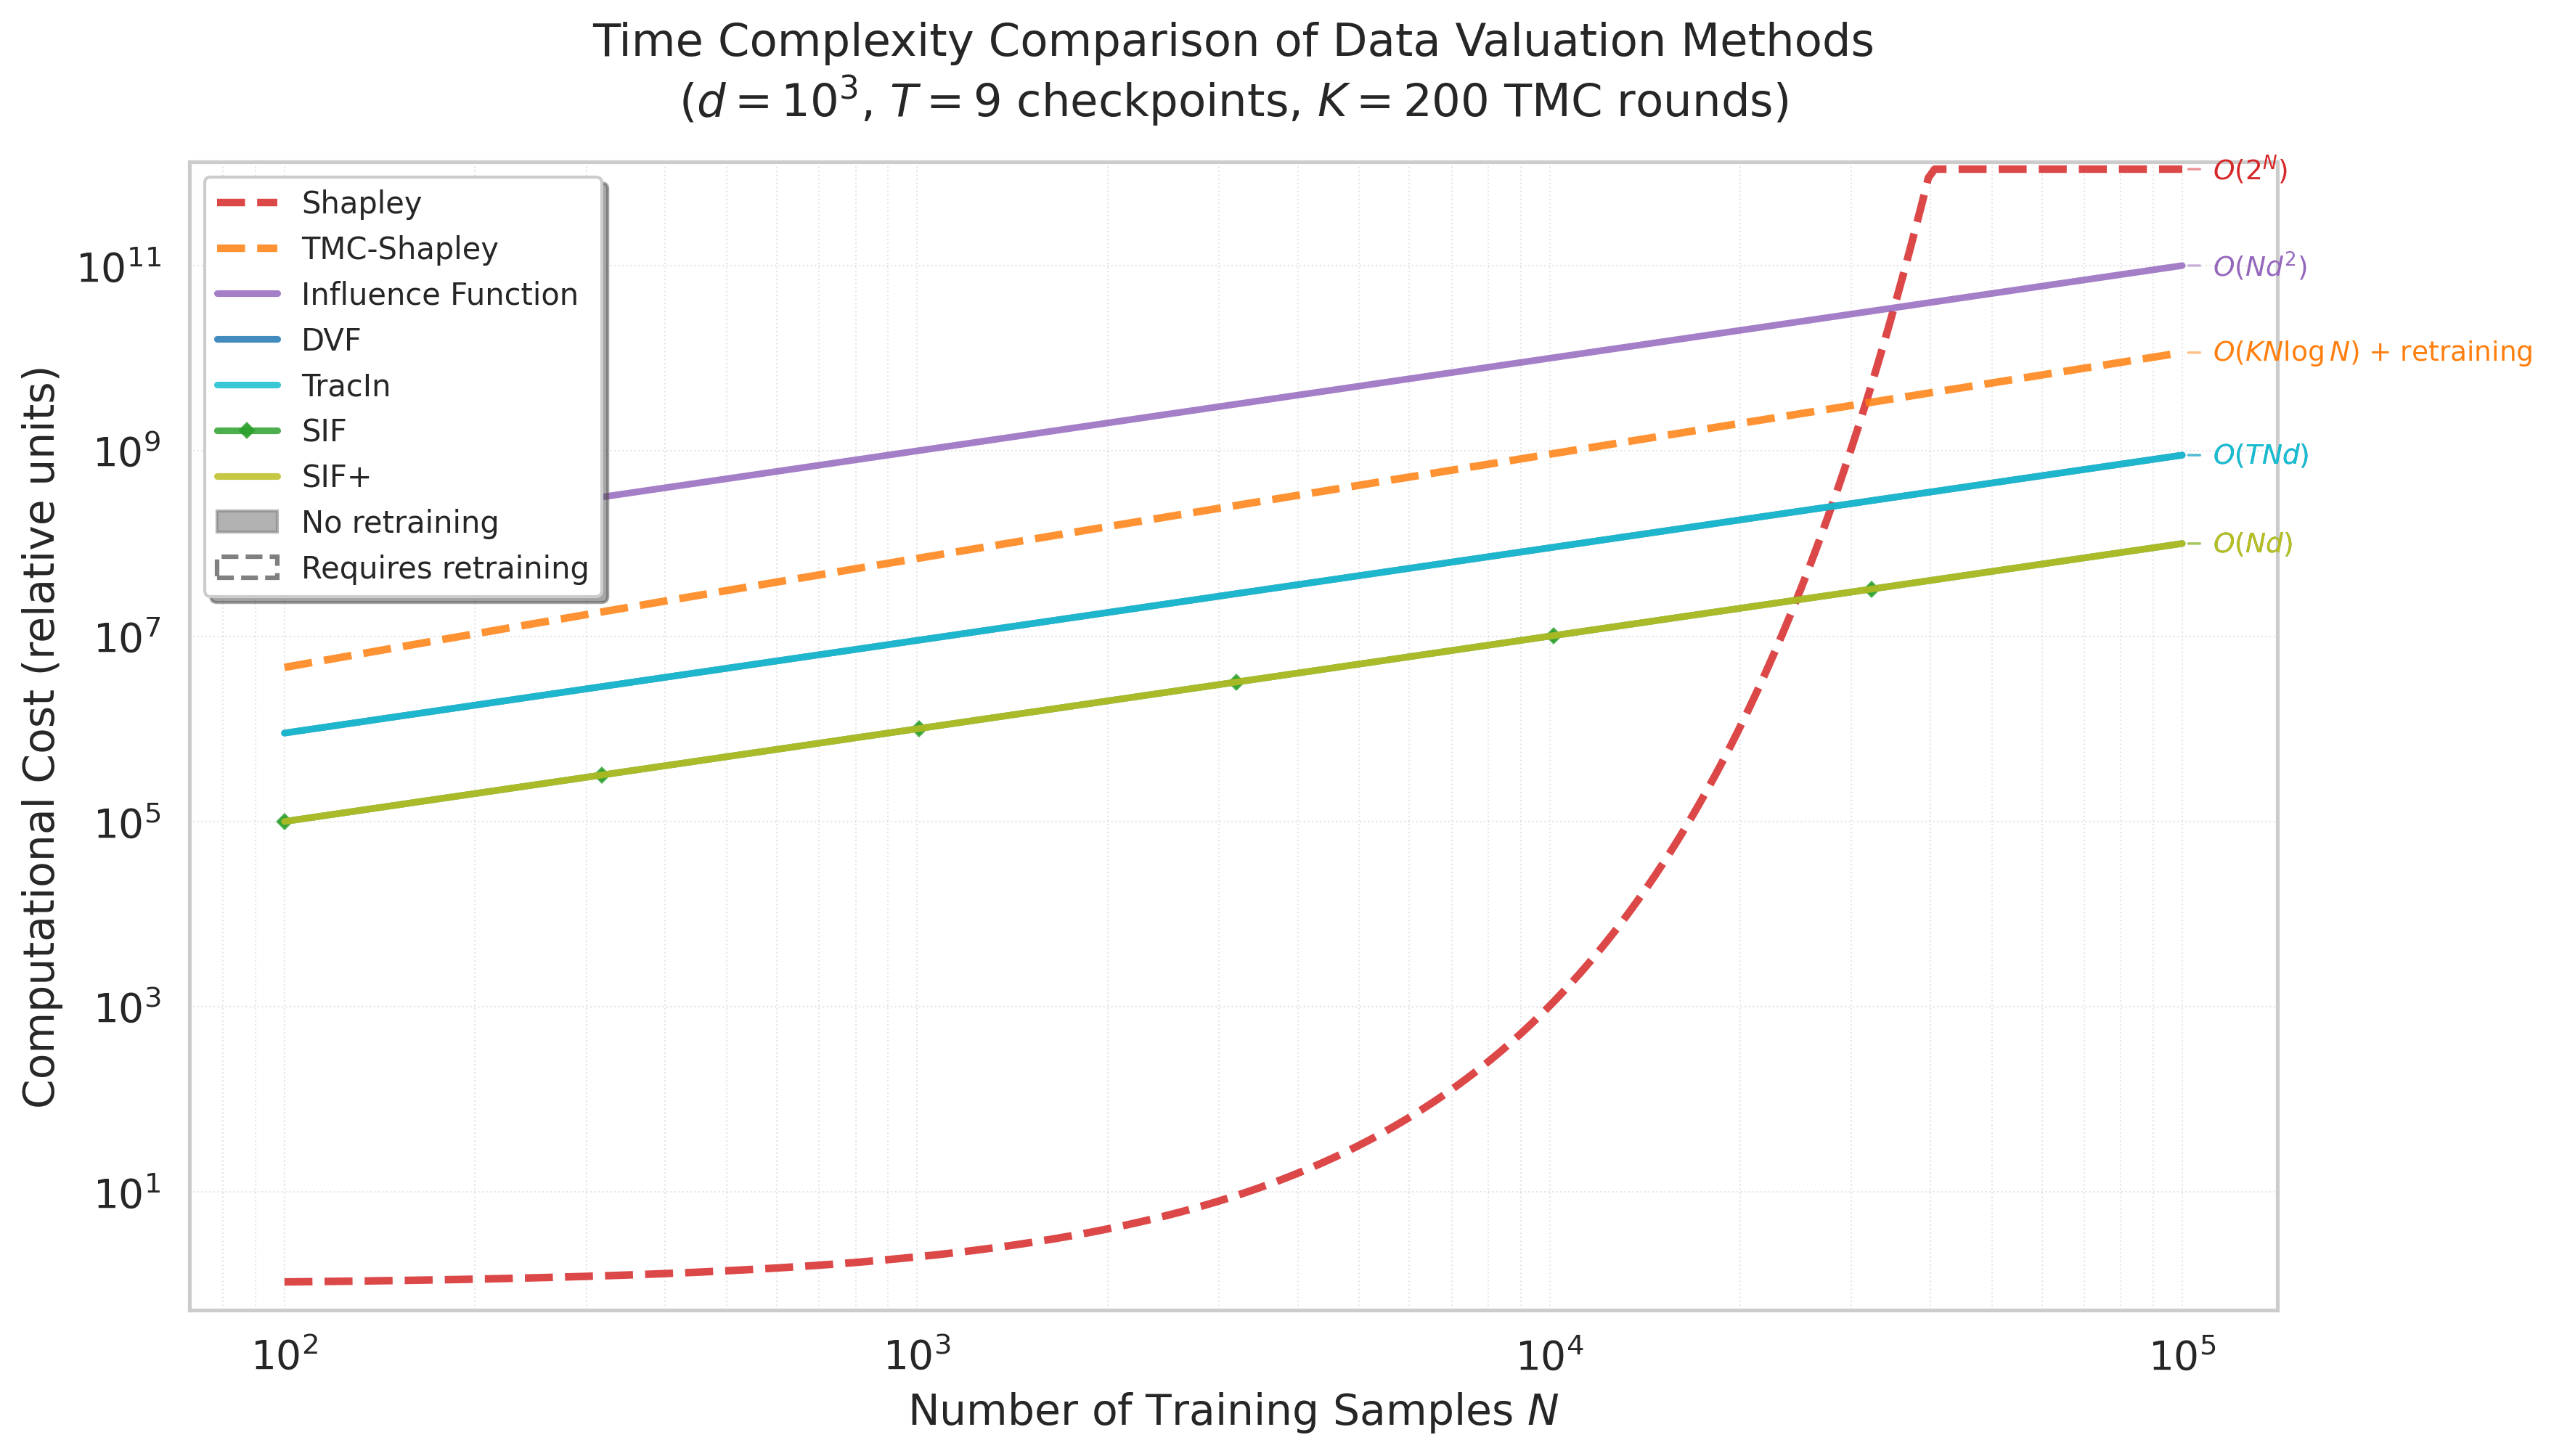
\includegraphics[width=0.8\linewidth]{complexity_comparison.png}
\caption{多种数据价值归因方法的计算复杂度比较}
\label{fig:complexity_comparison}
\end{figure}

\subsection{因果一致性的基线设定}

SHAP 在样本级归因场景下通常依赖大量子集采样或重复训练，在相同算力预算下其估计方差与耗时明显更高，不利于与轨迹类方法进行等成本比较。故为确保归因比较具备方法学一致性，本文不使用 SHAP\cite{lundberg2017unified}，而将 Influence Function、DVF 与 TracIn 设定为三类主基线（表\ref{tab:baseline}）。三者分别代表局部二阶近似、沿训练轨迹的动态累计影响以及离散检查点梯度追踪视角，可用于与本文提出的方法形成互补对照。
\begin{table}[htbp]
\centering
\caption{归因方法基线设定}
\label{tab:baseline}
\begin{tabular}{|p{4cm}|p{6cm}|p{4cm}|}
\hline
\textbf{基线类型} & \textbf{定义与方法} & \textbf{目的} \\
\hline
Influence Function（影响函数） & 基于验证损失对训练样本扰动的二阶近似，采用可计算的 Hessian 逆近似实现 & 提供局部灵敏度视角的归因基线 \\
\hline
DVF（Data Value Flow） & 沿训练轨迹累积验证梯度与样本梯度内积，刻画样本对泛化目标的动态影响 & 提供过程化、时序化的归因基线 \\
\hline
TracIn & 基于离散检查点的梯度内积求和估计样本影响，避免显式 Hessian 求逆 & 提供高效可扩展的轨迹追踪基线 \\
\hline
\end{tabular}
\end{table}

在实现层面，Influence Function 基线用于评估样本扰动对验证目标的局部影响强度，DVF 与 TracIn 基线用于评估沿训练轨迹的累计影响。本文方法则在此基础上比较不同轨迹近似与计算代价下的性能差异。

通过将DVF框架与分层数据资产结构以及基线体系相结合，我们获得了一个完整的流程，能够将宏观业务效益因果追溯到微观数据单元，从而实现数据资产的精细化管理与财务估值。

% ---------- 实验设计与仿真验证 ----------
\section{实验设计与仿真验证}
\label{sec:experiment}
\subsection{实验方法总览}
本节先对多源数据进行统一字段映射、样本过滤与张量化缓存构建，再在统一超参数口径下训练MLP基准推荐模型并以验证集指标监控训练过程，随后计算 SIF、Influence Function、TracIn 与 DVF 的样本级分数，并在统一 benchmark 协议下通过 deletion/insertion/NDCG 曲线及其面积指标、随机基线校正与多种子统计检验联合评估方法效果，从而在“可比性、可解释性与可复核性”三个维度形成闭环。

\subsection{数据来源}
本文实验数据采用三类公开推荐基准数据：MovieLens1M、Yahoo!Music 子集与 Pinterest 子集。为保证跨方法比较的公平性，本文在同一数据来源下执行统一字段映射与预处理。

\subsection{阶段一：统一数据准备与缓存}
在数据准备阶段，首先将不同公开推荐数据的原始交互字段统一映射为 user-item-label 三元表示，并通过最小交互阈值过滤稀疏噪声样本；随后构建训练/验证划分及样本标识，生成统一的张量化缓存（含稀疏特征、稠密特征、标签与样本ID），用于后续模型共享输入接口。该阶段的设计目标是避免数据格式差异对归因结论产生干扰。

\subsection{阶段二：MLP基准推荐模型训练}
在统一输入表示上，训练 MLP 基准推荐模型，并采用一致的训练设置（学习率、批大小与验证划分比例）。训练过程中按 epoch 记录验证损失、准确率与AUC，确保后续归因比较在统一评测口径下进行。

\subsection{阶段三：SIF与阶段DVF估值}
在完成基准训练后，基于保存的模型状态计算样本级价值分数。具体地，SIF以样本梯度与验证梯度内积作为一次性代理分数；阶段DVF则在多个训练阶段快照上累计样本影响，并输出总价值与分阶段价值（stage1、stage2），用于刻画数据价值在训练过程中的时序变化。该阶段输出样本级估值表及高/低价值样本列表，支持后续解释分析。

\subsection{阶段四：小样本归因对比验证}
为验证估值指标的有效性，进一步在小样本设置下进行归因对比实验：先从训练与验证集合中分别抽取固定规模子集，并在该子集上按统一效用函数生成各方法样本排序；再基于排序计算 deletion 曲线、insertion 曲线与 NDCG@Ke 曲线，并积分得到 deletion\_auc、insertion\_auc 与 ndcg\_ke\_auc，同时报告 pos@10 与方法耗时。为控制排序随机性的影响，实验对随机排序进行重复采样并构建随机参考值，最终同时报告原始指标与相对随机基线增益指标。

\subsection{方法实现与复现说明}
上述四阶段流程采用模块化实现：共享函数负责数据解析、模型构建与估值算子，流程层负责顺序执行与中间结果落盘。该实现方式使实验步骤、关键超参数与输出产物具备可追踪性，便于复现实验与开展增量对比。

\subsection{验证口径}
本文在实验验证中采用以下的统一设置：
\begin{itemize}
    \item \textbf{数据划分与子样本预算：}按随机种子进行 train/val 划分（val\_ratio=$0.2$，batch\_size=$256$），并在评测阶段固定子样本规模（$n\_{train}=96$、$n\_{val}=256$）以控制计算预算。
    \item \textbf{效用函数构造：}在训练子样本子集上执行短程重训练（epochs\_in\_utility=$14$，lr=$1\times10^{-3}$），以验证集 AUC 作为效用值，并通过重复训练取平均降低估计方差。
    \item \textbf{曲线与面积指标：}在 deletion\_fracs 与 insertion\_fracs（$\{0.05,0.1,0.2,0.3,0.4\}$）上计算 deletion/insertion 曲线及 AUC，在 ndcg\_ke（$\{5,10,20\}$）上计算 NDCG 曲线并积分得到 ndcg\_ke\_auc，同时报告 pos@10。
    \item \textbf{随机基线校正：}随机排序重复采样（random\_repeats=$7$），并以中位数聚合得到随机参考值；主结果同时报告原始指标与减随机基线增益指标。
    \item \textbf{多随机种子统计：}采用 $5$ 个随机种子重复实验，报告 mean$\pm$std，并对 SIF 与 Influence Function、DVF、TracIn 的差异使用 Wilcoxon signed-rank 检验与 Cliff's $\delta$ 效应量检验。
\end{itemize}

该验证口径对应“先训练并固定检查点，再在统一子样本预算下进行归因与反事实曲线评估”的流程，确保不同方法在同一训练产物与同水平评测预算下比较。

\subsection{结果边界与后续工作说明}
为避免读者对当前结果的解释范围产生误解，本文声明：主文报告已完成实验部分对应的证据范围；对于尚在推进中的部分，我们在此仅给出后续验证计划，不将其提前写入正文的结论。
\begin{itemize}
    \item \textbf{解释边界：}本文将结果定位为趋势性证据（trend-level evidence）；对未达到校正后显著性门槛的比较，不作确定性优越判断。
    \item \textbf{评测一致性：}后续补充实验将保持同一评测协议（seed 方案、随机基线聚合、Wilcoxon 与 Holm 校正、Cliff's $\delta$），以保证不同阶段结果可比。
    \item \textbf{可追踪披露：}新增结果将以“时间戳+配置快照+输出文件清单”的方式给出，便于读者核对差异来源。
    \item \textbf{完整呈现：}后续报告将同时呈现显著与不显著结果，尽量降低选择性展示带来的偏差。
\end{itemize}


\subsection{主结果}
本节给出到本文截稿日为止的有效实测结果。表 \ref{tab:main_result} 中指标来自同一评测口径下的 5 个随机种子统计，数值以 mean$\pm$std 形式报告；统计列基于 Wilcoxon 检验与 Holm 校正结果。

\begin{table}[htbp]
\centering
\caption{主结果（一）：归因质量与运行耗时（MLP，5 seeds，mean$\pm$std）}
\label{tab:main_result}
\small
\begin{tabular}{@{}lcccc@{}}
\toprule
方法 & Deletion-AUC$\uparrow$ & Insertion-AUC$\uparrow$ & NDCG@Ke-AUC$\uparrow$ & 用时(s)$\downarrow$ \\ \midrule
SIF             & $0.0669\pm0.0248$ & $0.1419\pm0.0334$ & $33.75\pm4.42$ & $1.1128\pm0.1776$ \\
SIF+            & $0.0683\pm0.0209$ & $0.1513\pm0.0216$ & $35.43\pm2.80$ & $1.3953\pm0.1099$ \\
Infl.\ Func.    & $-0.0091\pm0.0066$ & $0.0689\pm0.0124$ & $27.20\pm7.59$ & $1.5431\pm0.1459$ \\
DVF             & $0.0691\pm0.0261$ & $0.1402\pm0.0385$ & $33.85\pm3.78$ & $27.8705\pm0.5167$ \\
TracIn          & $0.0689\pm0.0257$ & $0.1408\pm0.0394$ & $33.89\pm3.68$ & $27.8701\pm0.5167$ \\ \bottomrule
\end{tabular}
\end{table}

\begin{table}[htbp]
\centering
\caption{主结果（二）：Wilcoxon 检验与 Holm 校正结果}
\label{tab:main_stat}
\small
\begin{tabular}{@{}lcc@{}}
\toprule
方法 & vs.\ SIF+（Holm $p$） & vs.\ SIF（Holm $p$） \\ \midrule
SIF             & 未显著（$p=1.000$）     & 参考方法 \\
SIF+            & 参考方法                & 未显著（$p=1.000$） \\
Infl.\ Func.    & 未显著（$p\geq0.625$） & 未显著（$p\geq0.625$） \\
DVF             & 未显著（$p=1.000$）     & 未显著（$p=1.000$） \\
TracIn          & 未显著（$p=1.000$）     & 未显著（$p=1.000$） \\ \bottomrule
\end{tabular}
\end{table}

\begin{figure}[H]
\centering
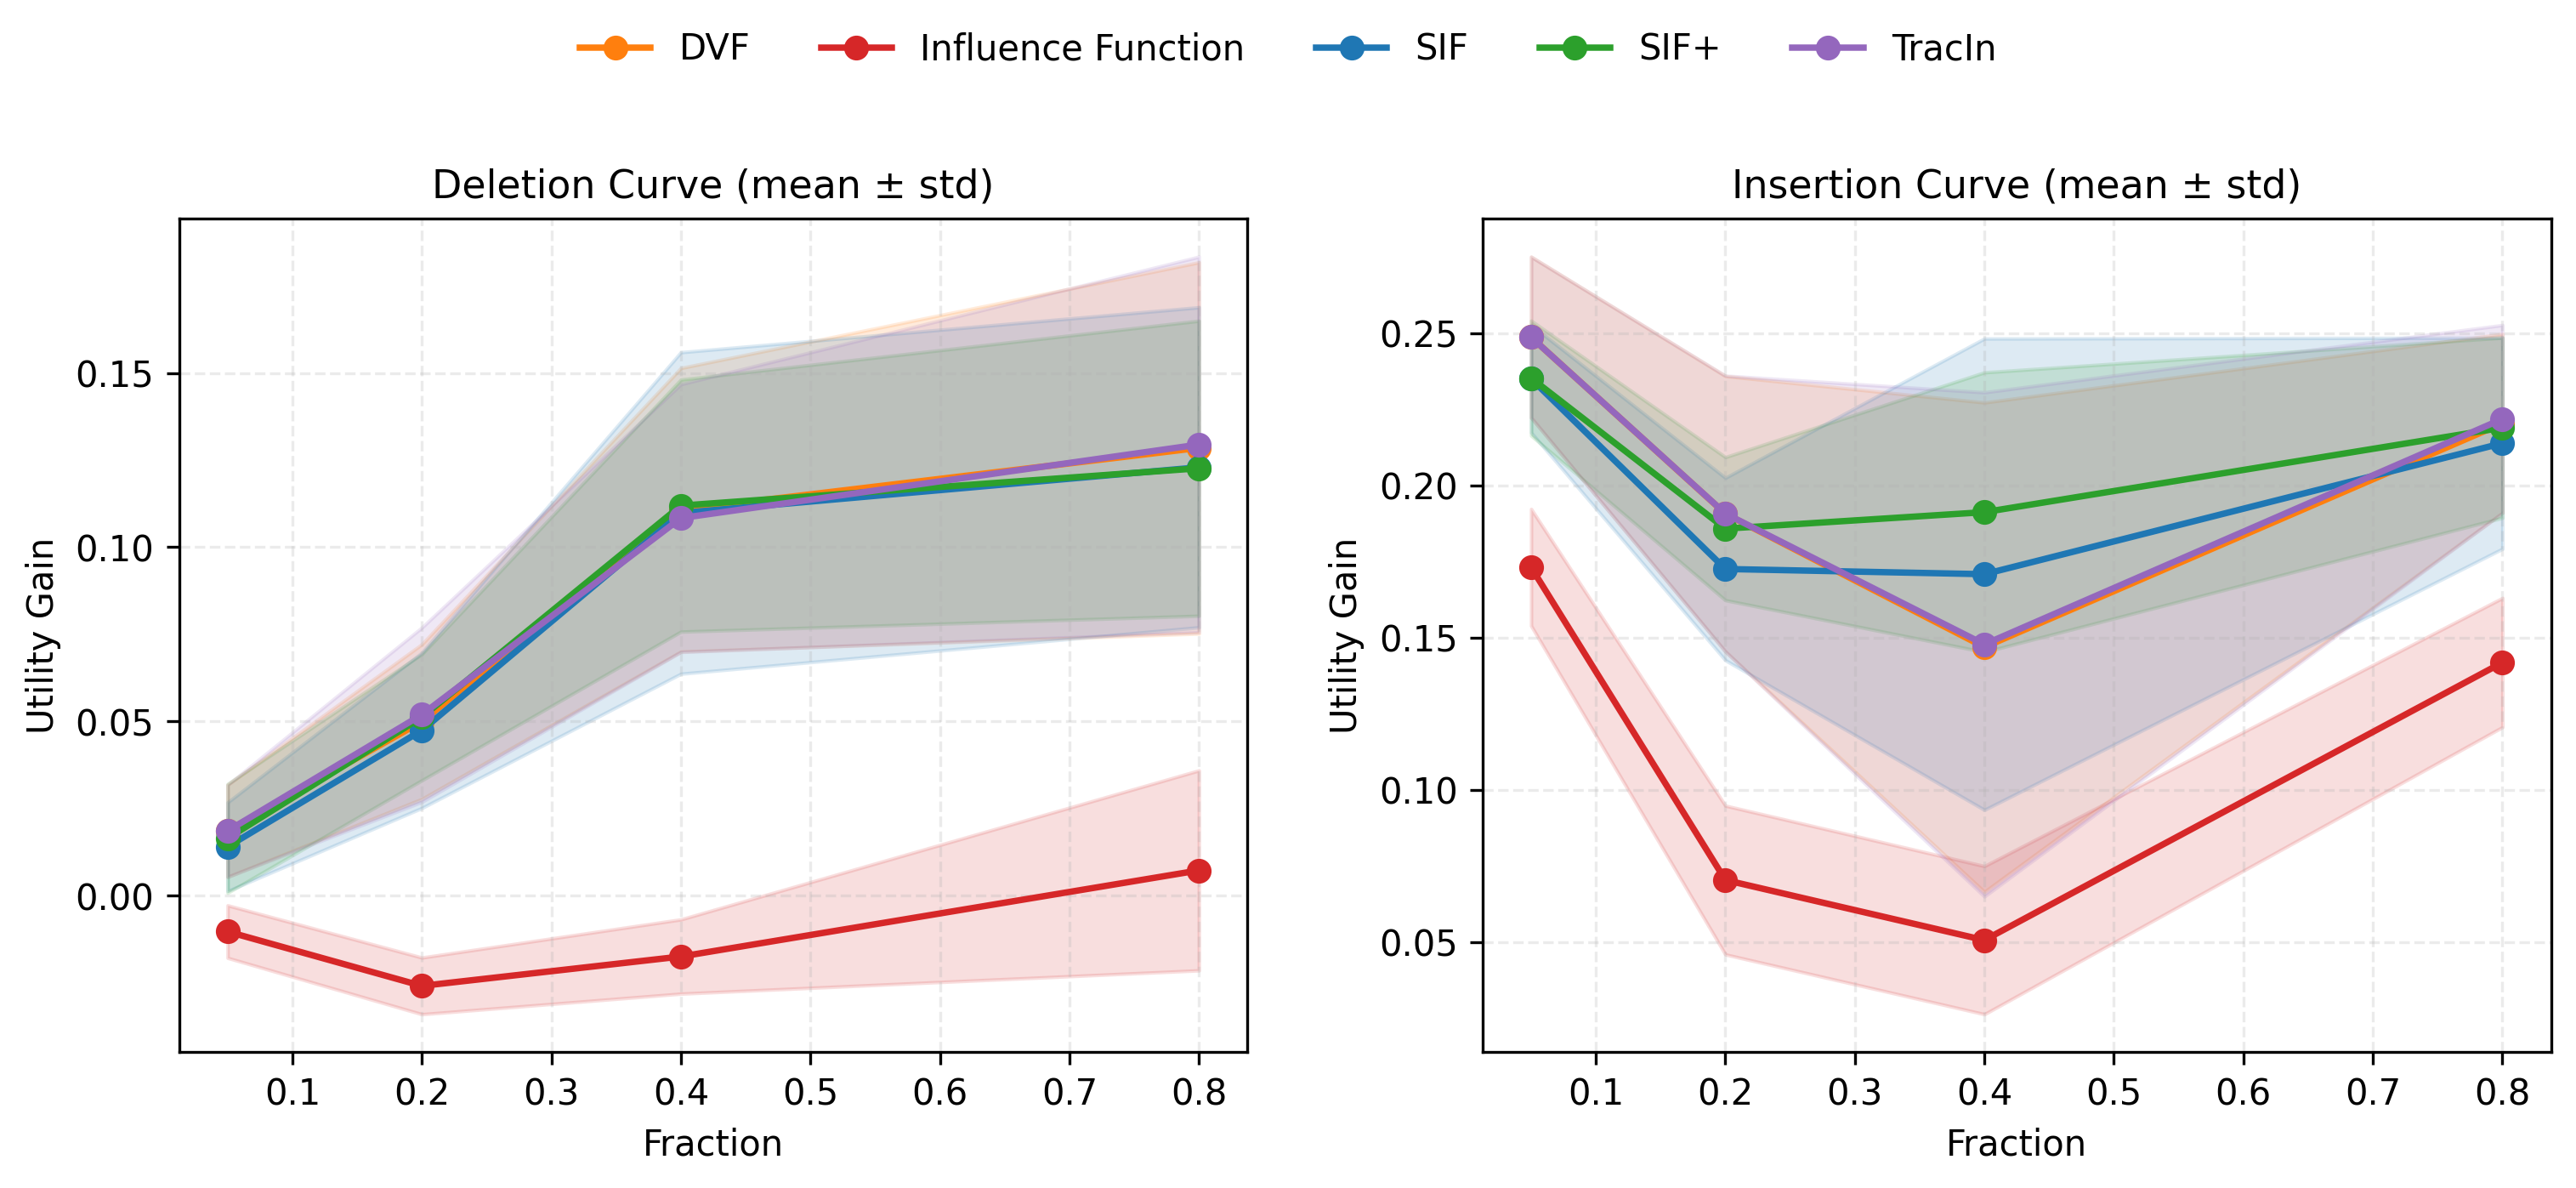
\includegraphics[width=\textwidth]{figures/del&ins_auc.png}
\caption{删除与插入AUC曲线}
\label{fig:del_ins_auc}
\end{figure}


% ---------- 结论 ----------
\section{结论}
\label{sec:conclusion}

本研究的结论以第6.9节结果表中的核心指标为依据：Deletion-AUC、Insertion-AUC、NDCG@Ke-AUC、相对随机基线增益（minus-random）、POS@10、运行耗时以及多随机种子下的统计检验（Wilcoxon 与 Cliff's $\delta$）。据此可归纳如下。

其一，当前结果支持如下\textbf{趋势性发现}：SIF/SIF+ 在计算开销与归因效果之间具有较优折中，能够在统一评测预算下提供可解释且可部署的样本级价值估计。

其二，考虑到当前样本规模等实验条件下部分比较尚未达到校正后显著性门槛，本文不将趋势性差异外推描述为确定性优越结论。

其三，本文把 VAE 与 NCF 作为后续完善验证模型，并在不变的统计口径下持续追加结果；后续版本仅在“方向一致 + 校正后显著 + 效应量充分”的条件下升级为强结论。

综上，本文当前提交版本完成了“理论框架 + 实证趋势 + 复现流程”的闭环，并为后续实证扩展提供了可审计、可持续更新的研究路径。

% ---------- 应用前景与讨论 ----------
\section{应用前景与讨论}
\label{sec:discussion}

\subsection{方法局限性分析}

SIF 与 SIF+ 的理论推导均依赖模型参数收敛至稳定点 $\theta^*$ 的假设（假设 A2）。在此假设下，验证梯度 $\nabla_\theta L_{\mathrm{val}}(\theta^*)$ 与样本梯度的内积能够稳定反映样本对泛化目标的边际贡献。然而，工业场景中出于防止过拟合或节省算力的考量，模型往往采用\textbf{早停策略}（early stopping），在损失尚未充分收敛时即终止训练。此时参数 $\theta_t$ 距离稳定点存在系统性偏差，导致以下问题：

\begin{itemize}
    \item \textbf{梯度方向不稳定：}早停点附近的验证梯度仍处于快速变化阶段，单次快照的内积估计方差较大，SIF 分数的跨样本排序可靠性下降。
    \item \textbf{曲率近似失效：}SIF+ 的对角 Hessian 近似在收敛邻域内具有理论保证，但在早停点处 Hessian 特征值分布可能尚未稳定，对角近似的误差界不再成立。
    \item \textbf{阶段分解偏移：}DVF 的阶段分解以梯度范数阈值 $\epsilon$ 划定表示学习与对齐阶段的边界，早停可能导致对齐阶段贡献被截断，低估后期训练样本的价值。
\end{itemize}

针对上述局限，一种可行的缓解策略是在早停点之后继续执行若干步"价值评估专用微调"（valuation fine-tuning），以较小学习率使模型在验证集上进一步收敛，再计算 SIF/SIF+ 分数；或采用多检查点平均策略，对早停前后若干检查点的 SIF 分数取加权均值，以降低单点估计的方差。这两种方案均可在不改变主训练流程的前提下提升早停场景下的估值稳定性，是本文方法在工程落地中需要重点关注的改进方向。

\subsection{商业应用价值}

本文框架的应用需严格遵循相关法律法规：
\begin{itemize}
    \item 《中华人民共和国个人信息保护法》第四条、第六条：原始行为日志（含user id）属于个人信息，但特征级embedding、统计特征、偏好向量经匿名化处理后不属于个人信息；本文不对完整用户画像整体定价，符合最小必要原则。
    \item 《中华人民共和国数据安全法》第二十七条：本文方案不对原始明细数据做外部流通，仅输出价值仪表盘，保障数据安全。
    \item 《互联网信息服务算法推荐管理规定》第十六条：归因过程使推荐算法的决策权重可追溯，增强了算法透明度。
\end{itemize}

在合规前提下，该框架可在以下三个维度释放商业价值：

\begin{itemize}
    \item \textbf{数据采购决策：}通过 SIF+ 分数量化不同来源数据对推荐效果的边际贡献，为数据采购谈判提供客观定价依据，避免"按量付费"模式下的价值错配。
    \item \textbf{数据资产仪表盘：}周期性输出样本级、实体级与数据集级价值报告，回答"本次促销增长主要归功于哪些数据"、"每TB用户行为数据的季度边际收益是多少"等具体管理问题，支撑数据要素的合规高效流通。
    \item \textbf{数据清洗与治理：}将持续低价值或负价值样本（SIF+ 分数显著为负）标记为噪声候选，辅助数据质量团队制定清洗优先级，在不损失模型效果的前提下降低存储与计算成本。
\end{itemize}

梯度信息存在模型反转攻击的隐私泄露风险。本文采用梯度加噪与差分隐私机制防护，系统仅输出\textbf{价值分数}，不输出原始数据与梯度，符合《个人信息保护法》《数据安全法》要求。

\subsection{未来工作展望}
本文实验部分正在持续完善中，后续版本将补充以下内容：
\begin{itemize}
    \item \textbf{模型多样性：}除 MLP 外，增加 VAE 与 NCF 作为验证模型，以测试方法在不同架构下的适用性与稳定性。
    \item \textbf{数据规模扩展：}在更大规模数据集（如 MovieLens 20M）上验证方法的可扩展性与效果趋势。
    \item \textbf{早停场景验证：}针对早停策略下的估值稳定性问题，设计专门的实验验证上述局限性分析中的缓解方案。
    \item \textbf{商业应用A/B测试：}在实际推荐系统中部署 SIF+ 作为数据价值监控工具，评估其对数据采购决策与清洗优先级制定的实际影响。
\end{itemize}
此外，未来工作还将探索更高阶的曲率近似方法（如 K-FAC）在 SIF+ 中的应用，以及将 DVF 与数据 Shapley 值的理论联系进一步形式化，以深化对数据价值评估方法之间关系的理解。积分梯度等公理化归因方法\cite{sundararajan2017axiomatic}与本文框架在归因公理层面存在潜在联系，亦是值得探索的理论延伸方向。本文实验代码与数据处理流程已开源\cite{repository}，以支持后续复现与扩展研究。

% ---------- 参考文献 ----------
\begin{thebibliography}{99}
\bibitem{repository}
项目仓库：\url{https://git.tsinghua.edu.cn/26tzb/recacc}

\bibitem{sundararajan2017axiomatic}
M. Sundararajan, A. Taly, and Q. Yan, "Axiomatic attribution for deep networks," in \textit{International Conference on Machine Learning (ICML)}, 2017, pp. 3319–3328.

\bibitem{lundberg2017unified}
S. M. Lundberg and S.-I. Lee, "A unified approach to interpreting model predictions,” in \textit{Advances in Neural Information Processing Systems (NeurIPS)}, 2017, pp. 4765–4774.

\bibitem{zhou2018deep}
G. Zhou, X. Zhu, C. Song, Y. Fan, H. Zhu, X. Ma, Y. Yan, J. Jin, H. Li, and K. Gai, "Deep interest network for click-through rate prediction,” in \textit{ACM SIGKDD International Conference on Knowledge Discovery \& Data Mining}, 2018, pp. 1059–1068.

\bibitem{shapley1953value}
L. S. Shapley, "A value for n-person games,” \textit{Contributions to the Theory of Games}, vol. 2, no. 28, pp. 307–317, 1953.

\bibitem{ghorbani2019data}
A. Ghorbani and J. Zou, "Data shapley: Equitable valuation of data for machine learning,” in \textit{International Conference on Machine Learning (ICML)}, 2019, pp. 2242–2251.

\bibitem{jia2019towards}
R. Jia, D. Dao, B. Wang, F. A. Hubis, N. Hynes, N. M. Gurel, B. Li, C. Zhang, D. Song, and C. Spanos, "Towards efficient data valuation based on the shapley value,” in \textit{International Conference on Artificial Intelligence and Statistics (AISTATS)}, 2019, pp. 1167–1176.

\bibitem{xu2023data}
J. Xu, N. Hong, Z. Xu, Z. Zhao, C. Wu, K. Kuang, J. Wang, M. Zhu, J. Zhou, K. Ren, X. Yang, C. Lu, J. Pei, and H. Shum, "Data-driven learning for data rights, data pricing, and privacy computing,” \textit{Frontiers of Information Technology \& Electronic Engineering}, vol. 24, no. 1, pp. 1–24, 2023.

\bibitem{influence}
Koh, P. W., \& Liang, P. (2017, July). Understanding black-box predictions via influence functions. In International conference on machine learning (pp. 1885-1894). PMLR.

\bibitem{TracIn}
Pruthi, G., Liu, F., Kale, S., \& Sundararajan, M. (2020). Estimating training data influence by tracing gradient descent. Advances in Neural Information Processing Systems, 33, 19920-19930.

\bibitem{StochasticApproximation}
Kushner, H. J., \& Yin, G. G. (2003). Stochastic approximation and recursive algorithms and applications. New York, NY: Springer New York.

\bibitem{andos2012computation}
Ando, K. (2012). Computation of the Shapley value of minimum cost spanning tree games:\# P-hardness and polynomial cases. Japan Journal of Industrial and Applied Mathematics, 29(3), 385-400.

\bibitem{zeiler2014visualizing}
Zeiler, M. D., \& Fergus, R. (2014, September). Visualizing and understanding convolutional networks. In European conference on computer vision (pp. 818-833). Cham: Springer International Publishing.
\end{thebibliography}

\end{document}